%
% File lfd1617.tex
%
%% Based on the style files for EACL-2017
%% Based on the style files for ACL-2016
%% Based on the style files for ACL-2015, with some improvements
%%  taken from the NAACL-2016 style
%% Based on the style files for ACL-2014, which were, in turn,
%% Based on the style files for ACL-2013, which were, in turn,
%% Based on the style files for ACL-2012, which were, in turn,
%% based on the style files for ACL-2011, which were, in turn,
%% based on the style files for ACL-2010, which were, in turn,
%% based on the style files for ACL-IJCNLP-2009, which were, in turn,
%% based on the style files for EACL-2009 and IJCNLP-2008...

%% Based on the style files for EACL 2006 by
%%e.agirre@ehu.es or Sergi.Balari@uab.es
%% and that of ACL 08 by Joakim Nivre and Noah Smith

\documentclass[11pt]{article}
\usepackage{eacl2017}
\usepackage{times}
\usepackage{url}
\usepackage{latexsym}
\usepackage{tikz}


%%%% LEAVE THIS IN
\eaclfinalcopy


\newcommand\BibTeX{B{\sc ib}\TeX}



\title{Learning from Data - Assignment 1 - Naive Bayes Classification}

\author{Remko Boschker \\
  master student of information science at the Rijks Universiteit Groningen \\
  {\tt s1282603, r.boschker@student.rug.nl} }

\date{}

\begin{document}
\maketitle
\begin{abstract}
This study compares the performance of naive Bayes, decision tree and k-nearest neighbour classification of a corpus of reviews by topic.
\end{abstract}

\section{Introduction}

This study attempts to find the best way to classify reviews by topic. I will analyse the performance of three methods and for each method I will try to find the optimal parameter settings. The methods are naive Bayes, decision tree and k-nearest neighbour classification. I will also analyse what representation of the documents gives the best performance. The representations I want to try are a vector containing the term frequency - inverse document frequency statistic for each word in the document and a sparse matrix containing per document all the counts for all the words in the corpus. For both the vectorisations I will experiment with lemmatisation of the input words and with a stop word list.

\section{Data}

The study uses a corpus of six thousand product reviews. Each review consists of a label indicating whether the review is positive or negative and a label indicating to which of the followings six topics it belongs: books, camera, dvd, health, music or software. The review also contains a file reference and the actual text of the review. The topic and sentiment labels are distributed almost equally across the corpus. About half of the reviews about a particular topic are labeled positive. Table ~\ref{tab:corpus} shows the counts for the labels in the corpus.

\begin{table}[h]\footnotesize
\label{tab:corpus}
\begin{tabular}{ l r r r r r r }
topic & cnt & \% & pos & \% & neg & \% \\
\hline
books & 993 & 16.5 & 471 & 47 & 522 & 53 \\
music & 1027 & 17.1 & 531 & 52 & 496 & 48 \\
dvd & 1012 & 16.9 & 490 & 48 & 522 & 52 \\
health & 986 & 16.4 & 470 & 48 & 516 & 52 \\
software & 994 & 16.6 & 502 & 51 & 492 & 49 \\
camera & 988 & 16.5 & 504 & 51 & 484 & 49 \\
\hline
total & 6000 & 100.0 & 2968 & 48 & 3132 & 52 \\
\end{tabular}
\caption{counts of topic and sentiment labels}
\end{table}

\section{Method/Approach}

This study compares the performance of the Scikit-learn implementations of three classification algorithms, Multinomial Naive Bayes, decision tree and k-nearest neighbour. First I compare the performance of the algorithms using default parameters but with different representations of the documents that need to be classified. Then I evaluate the effect of tuning the parameters of the algorithms using the best performing document representation. In this way I limit the number of combinations that need to be evaluated. I do not investigate feature selection methods.

I measure the performance in terms of precision, accuracy, f1-score and the time it takes to train and test the models using four-fold cross-validation. I use the cross-validation to predict all topic labels first and then I calculate the scores. The score I use in the evaluation is the weighted average of the scores for the prediction of each of the six labels. The duration is to time it takes for all four cross validation runs to complete training and predicting. The runs are run in parallel on a computer with 16 GB of RAM and a 2.6 GHz quad core Intel i7 processor.

\section{Optimising Representations}

I compare twelve different representations. They are generated using either the TF-IDF or Count vectoriser from the Scikit-learn Python library. Both vectorisers can be used with or without lemmatisation or stemming and with or without the default stop word list for English included with the library. I use the \emph{PorterStemmer} and \emph{WordNetLemmatizer} from the Scikit-learn library. The \emph{WordNetLemmatizer} requires that the word is tagged as a noun, verb, adjective or adverb. I use the NLTK POS-tagger and then map the resulting Penn Treebank POS-tags to these four categories.

\begin{table*}[h]\footnotesize
\centering
\label{tab:scores-repres-bayes}
\begin{tabular}{ l l l l l l l }
vectoriser & preprocessor & stop words & duration & precision & recall & f1-score \\
\hline
tf-idf & lemmatise & english & 2.5min & 0.9113 & 0.9087 & 0.9085 \\
tf-idf & none & english & 1.6s & 0.9089 & 0.9058 & 0.9056 \\
tf-idf & stem & english & 22.8s & 0.9080 & 0.9050 & 0.9048 \\
count & stem & english & 22.5s & 0.9049 & 0.9023 & 0.9022 \\
count & none & english & 1.6s & 0.9045 & 0.9015 & 0.9012 \\
count & lemmatise & english & 2.7min & 0.9038 & 0.9010 & 0.9008 \\
tf-idf & stem & none & 23.4s & 0.9036 & 0.8988 & 0.8986 \\
count & stem & none & 22.9s & 0.9004 & 0.8972 & 0.8972 \\
tf-idf & lemmatise & none & 2.8min & 0.9019 & 0.8968 & 0.8966 \\
count & lemmatise & none & 2.9min & 0.8997 & 0.8955 & 0.8955 \\
tf-idf & none & none & 2.0s & 0.9006 & 0.8953 & 0.8950 \\
count & none & none & 2.2s & 0.8966 & 0.8918 & 0.8916 \\
\end{tabular}
\caption{scores for different representations and the naive Bayes classifier sorted by f1-score}
\end{table*}

Table~\ref{tab:scores-repres-bayes} shows the results of running the classification task using the naive Bayes with the twelve document representations mentioned. The results are sorted by f1-score. The difference between the highest and lowest score is only 0.0169. Using stop words to exclude words from the feature vector consistently improves the score by 0.0053 to 0.0113. Within the scores using the stop words the tf-idf vectoriser performs bettern than the count vectoriser. Lemmatising improves the score for the tf-idf vectorisation and stemming for the count vectorisation. The lemmatising increases the duration by at least a factor twenty. I will use the highest scoring representation, with a f1-score of 0.9085 for the experiments with parameter tuning. This representation is the tf-idf vectorisation of the documents that was filtered by stop words and lemmatised.

\begin{table*}[h]\footnotesize
\centering
\label{tab:scores-repres-tree}
\begin{tabular}{ l l l l l l l }
vectoriser & preprocessor & stop words & duration & precision & recall & f1-score \\
\hline
count & lemmatise & english & 2.9min & 0.8115 & 0.8073 & 0.8087 \\
count & none & english & 5.0s & 0.8120 & 0.8065 & 0.8081 \\
count & stem & english & 25.6s & 0.8053 & 0.8008 & 0.8023 \\
tf-idf & none & english & 6.0s & 0.8010 & 0.7957 & 0.7974 \\
tf-idf & lemmatise & english & 2.6min &  0.7982 & 0.7940 & 0.7955 \\
count & stem & none & 26.7s & 0.7934 & 0.7917 & 0.7924 \\
tf-idf & stem & english & 25.8s & 0.7939 & 0.7905 & 0.7917 \\
count & lemmatise & none & 2.6min & 0.7926 & 0.7905 & 0.7912 \\
count & none & none & 6.4s & 0.7911 & 0.7870 & 0.7883 \\
tf-idf & stem & none & 29.2s & 0.7773 & 0.7763 & 0.7767 \\
tf-idf & lemmatise & none & 3.1min & 0.7739 & 0.7730 & 0.7733 \\
tf-idf & none & none & 8.1s & 0.7705 & 0.7680  & 0.7689 \\
\end{tabular}
\caption{scores for different representations and the decision tree classifier sorted by f1-score}
\end{table*}

The results for decision tree classifier are listed in table \ref{tab:scores-repres-tree}. The difference between the lowest and highest f1-score is larger than for the Naive Bayes classifier. It is 0.0398. Again the stop words improve the score 0.0150 to 0.0185. In contrast to the Bayes classifier the decision tree classifier performs better with the count vectorisation. The effect of stemming is not very clear. The highest scoring run used lemmatisation. I will use the representation with the highest f1-score of 0.8087. It is the count vectorisation of the lemmatised document first filtered on stop words.

\begin{table*}[h]\footnotesize
\centering
\label{tab:scores-repres-neighbour}
\begin{tabular}{ l l l l l l l }
vectoriser & preprocessor & stop words & duration & precision & recall & f1-score \\
\hline
tf-idf & stem & english & 23.8s & 0.8073 & 0.8048 & 0.8042 \\
tf-idf & lemmatise & english & 2.6min & 0.7998 & 0.7958 & 0.7953 \\
tf-idf & stem & none & 24.6s & 0.7903 & 0.7837 & 0.7835 \\
tf-idf & none & english & 3.9s & 0.7835 & 0.7780 & 0.7773  \\
tf-idf & lemmatise & none & 2.6min & 0.7767 & 0.7658 & 0.7660 \\
tf-idf & none & none & 4.3s & 0.7489 & 0.7340 & 0.7339 \\
count & stem & english & 23.6s & 0.5627 & 0.5455 & 0.5416 \\
count & lemmatise & english & 2.6min & 0.5555 & 0.5352 & 0.5301 \\
count & none & english & 3.2s & 0.4923 & 0.4775 & 0.4700 \\
count & stem & none &  24.6s & 0.4798 & 0.4622 & 0.4569 \\
count & lemmatise & none & 2.7min & 0.4630 & 0.4520 & 0.4448 \\
count & none & none & 4.3s & 0.4361 & 0.4232 & 0.4158 \\
\end{tabular}
\caption{scores for different representations and the k-nearest neighbour classifier sorted by f1-score}
\end{table*}

Table~\ref{tab:scores-repres-neighbour} listing the results for the k-nearest neighbour classifier shows the largest difference in the f1-score. The highest score, 0.8042 is nearly twice the lowest score of 0.4158. The tf-idf vectorisation scores works better then count vectorisation and the effect of the stop words is less clear. Still the two highest scores make use of the stop word list filter. Both vectorisations perform better with the Porster stemmer than with the lemmatisation. The best performing vectorisation uses the tf-idf statistic on the stemmed document without stop words. It has a f1-score of 0.8042 and it will be used for the parameter tuning experiments.

In summary, say something about the duration

\section{Tuning Classification Algorithm Parameters}

laplace = 1, 0 < 1 lidstone

1, true 2.5min & 0.9113 & 0.9087 & 0.9085 \\
1, false 3.3min 0.9114    0.9088    0.9086
0.5, false 3.5min 0.9101    0.9082    0.9081
0.5, true 3.2min 0.9093    0.9073    0.9072
1.5, true 3.3min 0.9091    0.9057    0.9053
1.5, false 3.2min 0.9093    0.9073    0.9072
1.1, false 3.2min 0.9115    0.9088    0.9086
0.9, false 3.0min 0.9114    0.9088    0.9087
0.8 false 3.0min 0.9103    0.9078    0.9077
0.1 false 2.7min 0.9034    0.9028    0.9027

alpha Additive (Laplace/Lidstone) smoothing parameter (0 for no smoothing).
fit prior true / false

Presorting is not supported for sparse matrices.

gini best none none 2 1 0 None 1e-7 False 2.8min 0.7988    0.7950    0.7964
entropy best none none 2 1 0 None 1e-7 False 2.6min 0.7873    0.7847    0.7857
gini random none none 2 1 0 None 1e-7 False 2.6min 0.7989    0.7957    0.7967
gini random sqrt none 2 1 0 None 1e-7 False 2.5min 0.5486    0.5473    0.5475
gini random log2 none 2 1 0 None 1e-7 False 2.6min 0.4041    0.4065    0.4049
gini random none 5 2 1 0 None 1e-7 False 2.6min 0.6808    0.4362    0.4282
gini random none 20 2 1 0 None 1e-7 False 2.7min 0.8203    0.7607    0.7717
gini random none 50 2 1 0 None 1e-7 False 2.6min 0.8268    0.7667    0.7772
gini random none 100 2 1 0 None 1e-7 False 2.6min 0.8080    0.8028    0.8043
gini random none 75 2 1 0 None 1e-7 False 2.6min 0.8035    0.7963    0.7985
gini random none 60 2 1 0 None 1e-7 False 2.6min 0.8207    0.8075    0.8104
gini random none 60 0.1 1 0 None 1e-7 False 2.6min 0.8022    0.7750    0.7773
gini random none 60 10 1 0 None 1e-7 False 2.6min 0.8089    0.7960    0.7993
gini random none 60 3 1 0 None 1e-7 False 2.6min 0.8161    0.8035    0.8064
gini best none 60 4 1 0 None 1e-7 False 2.8min 0.8210    0.8123    0.8146
gini best none 60 5 1 0 None 1e-7 False 2.6min 0.8210    0.8115    0.8139
gini best none 60 4 10 0 None 1e-7 False 2.6min 0.8001    0.7938    0.7955
gini best none 60 4 5 0 None 1e-7 False 2.6min 0.8059    0.8008    0.8023
gini best none 60 4 2 0 None 1e-7 False 2.7min 0.8096    0.8003    0.8027
gini best none 60 4 1 0 10 1e-7 False 2.6min 0.8212    0.7118    0.7253
gini best none 60 4 1 0 100 1e-7 False 2.6min 0.8335    0.8167    0.8203
gini best none 60 4 1 0 200 1e-7 False 2.6min 0.8271    0.8145    0.8176
gini best none 60 4 1 0 50 1e-7 False 2.6min 0.8401    0.8103    0.8158
gini best none 60 4 1 0 75 1e-7 False 2.6min 0.8323    0.8132    0.8173
gini best none 60 4 1 0 150 1e-7 False 2.8min 0.8322    0.8187    0.8218
gini random none 60 4 1 0 150 1e-7 False 2.7min 0.8262    0.8100    0.8134

criterion gini / entropy gini
splitter best /random best
max_features none
max_depth none
min_samples_split 2
min_samples_leaf 1
min_weight_fraction_leaf 0
random state None
min_impurity_split 1e-7
presort False




maximum number of leaves
minimum number of samples per leaf

knearest

weight uniform distance
algorithm ball_tree kd_tree brute auto
metric minkowski p=2 eql euclidean
p
n_jobs 4

all brute because sparse features

neighbours weights algorithm leaf_size metric p
3 uniform auto 30 minkowski 2 2.8min 0.5441    0.5062    0.4978
5 uniform auto 30 minkowski 2 2.8min 0.5555    0.5352    0.5301
7 uniform auto 30 minkowski 2 2.6min 0.5832    0.5537    0.5513
9 uniform auto 30 minkowski 2 2.6min  0.5881    0.5568    0.5556
11 uniform auto 30 minkowski 2 3.1min 0.6021    0.5625    0.5643
13 uniform auto 30 minkowski 2 2.6min  0.6083    0.5682    0.5697
15 uniform auto 30 minkowski 2 2.7min 0.6158    0.5698    0.5720
17 uniform auto 30 minkowski 2 2.7min 0.6208    0.5722    0.5744
19 uniform auto 30 minkowski 2 2.6min 0.6266    0.5735    0.5774
21 uniform auto 30 minkowski 2 3.0min 0.6350    0.5795    0.5839
49 uniform auto 30 minkowski 2 2.7min 0.6689    0.5823    0.5946
55 uniform auto 30 minkowski 2 3.1min 0.6696    0.5788    0.5909
63 uniform auto 30 minkowski 2 2.9min 0.6797    0.5753    0.5893
81 uniform auto 30 minkowski 2 2.6min 0.6745    0.5632    0.5791
121 uniform auto 30 minkowski 2 2.8min 0.6764    0.5428    0.5617
49 distance auto 30 minkowski 2 2.8min 0.6903    0.6055    0.6204
49 distance brute 15 minkowski 2 3.0min  0.6903    0.6055    0.6204
49 distance brute 45 minkowski 2 3.0min  0.6903    0.6055    0.6204
49 distance auto 30 minkowski 1 3.4min 0.7226    0.6507    0.6644

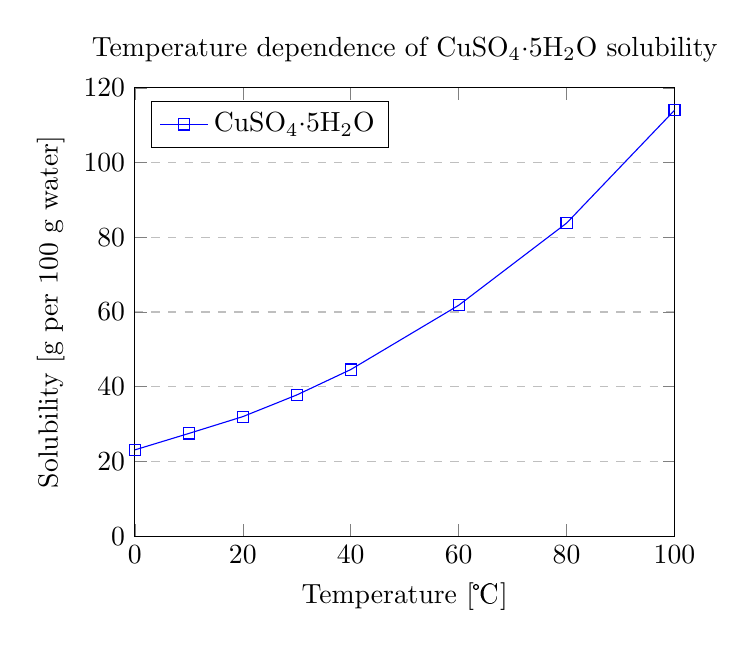
\begin{tikzpicture}
\begin{axis}[
    title={Temperature dependence of CuSO$_4\cdot$5H$_2$O solubility},
    xlabel={Temperature [\textcelsius]},
    ylabel={Solubility [g per 100 g water]},
    xmin=0, xmax=100,
    ymin=0, ymax=120,
    xtick={0,20,40,60,80,100},
    ytick={0,20,40,60,80,100,120},
    legend pos=north west,
    ymajorgrids=true,
    grid style=dashed,
]

\addplot[
    color=blue,
    mark=square,
    ]
    coordinates {
    (0,23.1)(10,27.5)(20,32)(30,37.8)(40,44.6)(60,61.8)(80,83.8)(100,114)
    };
    \legend{CuSO$_4\cdot$5H$_2$O}

\end{axis}
\end{tikzpicture}


\section{Results}

\section{Discussion/Conclusion}



\section{Answers to additional questions}

\subsection{decision tree theory}

To build the decision tree for the given example with the least amount of nodes you need to branch on the test with the highest information gain first. Information gain is the expected reduction in entropy for the \emph{edible} label in the example for sorting on either the \emph{color}, \emph{size} or \emph{shape} labels. The information gain is calculated by calculating the entropy for the parent set and subtracting the weighted average entropy of the child sets resulting from splitting on the label. The entropy of a set is calculated by $\sum\limits_i - p_i \log_2 p_i $ where $p_i$ is the probability of an element being in class \emph{i} modeled as the portion of the elements in the set being of class \emph{i}. The information gain achieved by sorting on the \emph{colour, size or shape} features is listed in table~\ref{tab:gain}. Sorting on the \emph{size} first achieves the highest gain and therefore this is what should be done first.

\begin{table}[h]\footnotesize
\label{tab:gain}
\begin{tabular}{ l r r r r r }
& \multicolumn{4}{c}{entropy} & \\
\cline{2-5}
label & parent & child1 & child2 & avg & gain \\
\hline
colour & 0.9886 & 0.9612 & 0.9182 & 0.9531 & 0.0355 \\
size & 0.9886 & 0.8112 & 0.9544 & 0.8828 & 0.1058 \\
shape & 0.9886 & 1 & 0.8112 & 0.9528 & 0.0358 \\
\end{tabular}
\caption{information gain on the first split with respect to the edible label}
\end{table}



\begin{table}[h]\footnotesize
\label{tab:gain-small}
\begin{tabular}{ l r r r r r }
& \multicolumn{4}{c}{entropy} & \\
\cline{2-5}
label & parent & child1 & child2 & avg & gain \\
\hline
colour & 0.8112 & 0.6500 & 1 & 0.7375 & 0.0737 \\
shape & 0.8112 & 0.9182 & 0 & 0.6887 & 0.1225 \\
\end{tabular}
\caption{information gain on the \emph{small} branch with respect to the edible label}
\end{table}

\begin{table}[h]\footnotesize
\label{tab:gain-large}
\begin{tabular}{ l r r r r r }
& \multicolumn{4}{c}{entropy} & \\
\cline{2-5}
label & parent & child1 & child2 & avg & gain \\
\hline
colour & 0.9544 & 0.9852 & 0 & 0.8620 & 0.0923 \\
shape & 0.9544 & 1 & 0.9182 & 0.9387 & 0.0157 \\
\end{tabular}
\caption{information gain on the \emph{large} branch with respect to the edible label}
\end{table}

\begin{figure*}
\label{fig:tree}
\caption{decision tree for predicting edible}
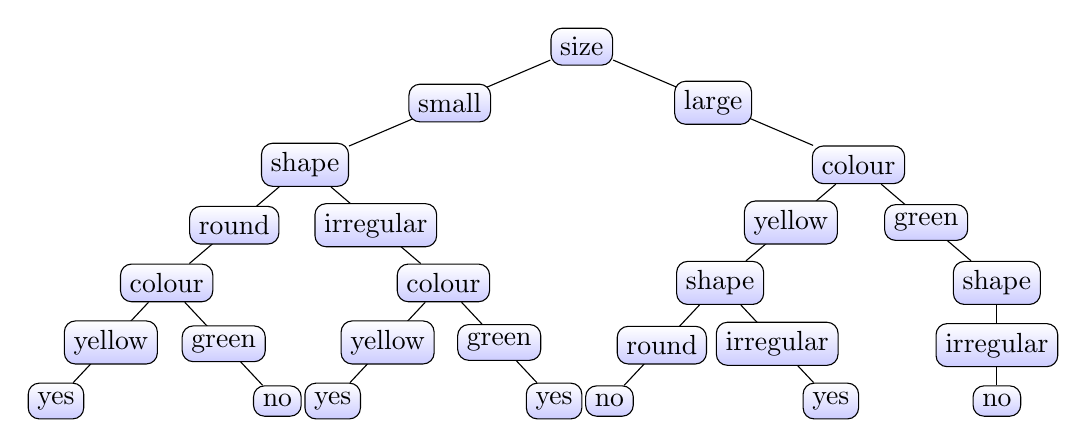
\begin{tikzpicture}[sibling distance=10em,
  every node/.style = {shape=rectangle, rounded corners,
    draw, align=center,
    top color=white, bottom color=blue!20},
  level 1/.style={sibling distance=20em},
  level 2/.style={sibling distance=10em},
  level 3/.style={sibling distance=8em},
  level 4/.style={sibling distance=8em}]
  \node {size}
    child { node {shape}
      child {node {colour}
        child {node {yes}
          edge from parent node {yellow}}
        child {node {no}
          edge from parent node {green}}
        edge from parent node {round}}
      child {node {colour}
        child {node {yes}
          edge from parent node {yellow}}
        child {node {yes}
          edge from parent node {green}}
        edge from parent node {irregular}}
      edge from parent node {small}}
    child { node {colour}
      child { node {shape}
        child { node {no}
          edge from parent node {round}}
        child { node {yes}
          edge from parent node {irregular}}
        edge from parent node {yellow}}
      child { node {shape}
        child { node {no}
          edge from parent node {irregular}}
        edge from parent node {green}}
      edge from parent node {large}};
\end{tikzpicture}
\end{figure*}

As can be seen in the tables ~\ref{tab:gain-small} and ~\ref{tab:gain-large} for the items labeled \emph{small} the next split with the most gain would be by \emph{shape} and for the items labeled large it would be \emph{colour}. The resulting tree is shown in figure ~\ref{fig:tree}. The leaf for items with the features \emph{yellow,  small, round} has a $\frac{4}{5}$ probability of being edible, but a $\frac{1}{5}$ probability of not being edible. There are no features to distinguish between them. The leaf was labeled with yes, because of the higher probability. The leaf for items with the features \emph{yellow,  large, round} was treated similarly labeling such items as not edible, although there is a $\frac{1}{5}$ probability that the item is edible. There is no item with the features \emph{green, large, round} and no branch for those features is included in the tree.

\bibliography{eacl2017}
\bibliography{yourbibfile}

\end{document}
